\documentclass[./main.tex]{subfiles}

\begin{document}
\section{Deep Learning Theory}
The following section covers the most important background theory for the experiments in Section \ref{sec:experiments}. This includes an introduction to various types of neural networks, as well as an introduction to the optimization of such networks.

\subsection{Feedforward Neural Networks}
\textbf{Feedforward neural networks} are the most basic type of neural networks. The aim of a feedforward neural network is to approximate some function $f^*$, by defining a mapping $\bm{y} = f(\bm{x}; \bm{\theta})$ and learning the parameters $\bm{\theta}$, that results in the best approximation of $f^*$. These models are called \textbf{feedforward} because there are no \textbf{feedback} connections in which the outputs of the model are fed back into itself. Instead, information flows through the function being evaluated from $\bm{x}$, through the intermediate computations used to define $f$, and finally to the output $\bm{y}$. Feedforward neural networks generally consists of multiple \textbf{layers}, arranged in a chain structure, with each layer being a function of the layer that preceded it \cite{DL_book}. 

\subsection{Fully-connected Layers}
The most simple type of layer found in a feeforward neural network is the \textbf{fully-connected layer}. The fully-connected layer usually consists of some learnable parameter matrix $\bm{W}$ and learnable parameter vector $\bm{b}$, as well as a non-linear \textbf{activation function} $g$ (which will be covered further in Section \ref{subsubsec:activation_func}). In this case, the $i$'th layer is defined as \cite{DL_book}
\begin{equation}
    \bm{h}^{(i)} =
    \begin{cases}
        g^{(i)} \left( \bm{W}^{(i) \top} \bm{h}^{(i)} + \bm{b}^{(i)} \right) & \text{if } i > 1 \\
        g^{(1)} \left( \bm{W}^{(1) \top} \bm{x} + \bm{b}^{(1)} \right) & \text{if } i = 1
    \end{cases}
    .
\end{equation}

\subsection{Convolutional Layer}
\begin{figure}[htbp]
    \centering
    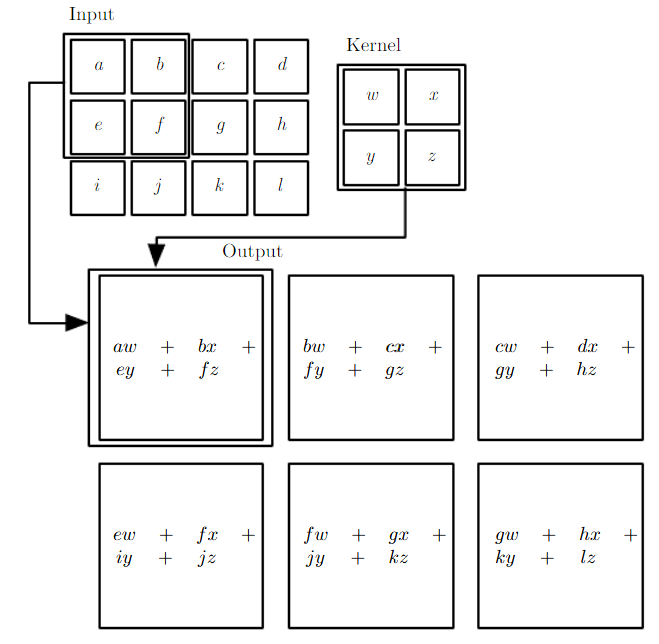
\includegraphics[width = 0.5 \textwidth]{./entities/2d_conv_example.PNG}
    \caption{An example of applying a 2d kernel on an input \cite{DL_book}.}
    \label{fig:2d_conv_example}
\end{figure}
A \textbf{convolutional layer} is a specialized kind of feedforward layer, usually used in analysis of time-series or image data \cite{DL_book}. If a network has at least one convolutional layer, it is called a \textbf{Convolutional neural network (CNN)}.
\\
\\
The convolutional layer consists of a set of \textbf{kernels}, each to be applied to the entire input vector, where each kernel is a learnable parameter matrix $k \times k$ \cite{everything}. Each kernel is applied on the input to produce a \textbf{feature map}. The kernels are applied to the input by "sliding" over the input (where the step size is called \textbf{stride}). Each $k \times k$ grid of the input is then used to compute the dot-product between the grid and each kernel, which is then placed in the corresponding feature map of each kernel, as visualized in Figure \ref{fig:2d_conv_example}. \cite{bsc_thesis}. To control the dimensions of the output, one might \textbf{pad} the sides with a constant value. Commonly, zero is used as the padding-value.
\\
\\
As seen in Figure \ref{fig:2d_conv_example}, each kernel produces a linear combination of all pixel values in a neighbourhood defined by the size of the kernel. Thus, unlike a fully-connected layer, a convolutional layer captures the high correlation between a pixel and its neighbours. Further, by limiting the size of the kernel, the network will use much fewer parameters, than if a fully-connected layer would be used instead \cite{DL_book}.



\subsection{Recurrent Neural Networks}
\subsubsection{Long Short-Term Memory Unit}
\begin{itemize}
    \item Convolutional LSTM
\end{itemize}
\subsubsection{Gated Recurrent Unit}
\begin{itemize}
    \item Convolutional GRU
\end{itemize}
\subsection{Transformer}
\subsection{Training a Neural Network}
\subsubsection{Activation function}
\label{subsubsec:activation_func}

\end{document}